\documentclass[]{article}
\usepackage{amssymb}
\usepackage{amsmath}
\usepackage{tikz}
\usetikzlibrary{decorations.markings}
\usetikzlibrary{backgrounds}
\usetikzlibrary{shapes, arrows, calc, arrows.meta, fit, positioning}
\tikzset{  
	-stealth,auto,node distance =1.5 cm and 1.3 cm, thick,% node distance is the distance between one node to other, where 1.5cm is the length of the edge between the nodes  
	state/.style ={circle, draw, inner sep=0.3pt}, % the minimum width is the width of the ellipse, which is the size of the shape of vertex in the node graph  
	point/.style = {circle, draw, inner sep=0.18cm, fill, node contents={}},  
	el/.style = {inner sep=2.5pt, align=right, sloped}  
}

\begin{document}

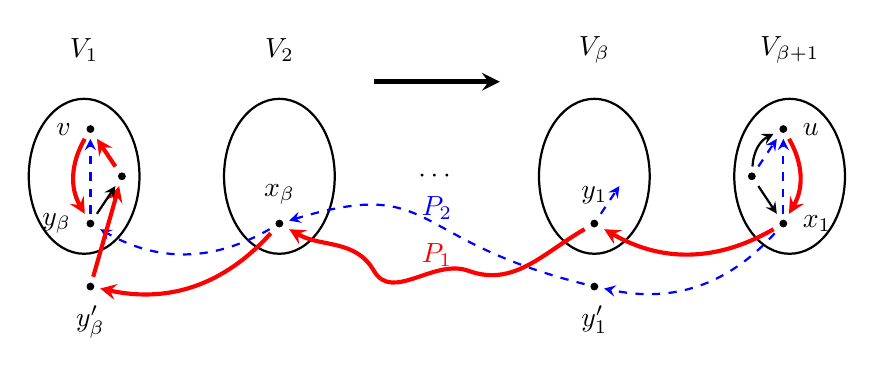
\begin{tikzpicture}[scale=0.4]
					\foreach \i in {(11.2,0),(5,0),(-5,0),(-11.2,0)}{\draw[ line width=0.8pt] \i ellipse [x radius=50pt, y radius=70pt];}
					\coordinate [label=center:$V_1$] () at (-11.2,4);
					\coordinate [label=center:$V_2$] () at (-5,4);
					\coordinate [label=center:$\cdots$] () at (0,0);
					\coordinate [label=center:{\color{red}$P_1$}] () at (0,-2.5);
					\coordinate [label=center:{\color{blue}$P_2$}] () at (0,-1);
					\coordinate [label=center:$V_\beta$] () at (5,4);
					\coordinate [label=center:$V_{\beta+1}$] () at (11.2,4);
					\draw[-stealth,line width=1.8pt] (-2,3) -- (2,3); 
					\filldraw[black](11,-1.5) circle (3pt)node[label=right:$x_1$](x1){};
					\filldraw[black](-11,-1.5) circle (3pt)node[label=left:$y_\beta$](yb){};
					\filldraw[black](-11,1.5) circle (3pt)node[label=left:$v$](v){};
					\filldraw[black](-5,-1.5) circle (3pt)node[label=above:$x_\beta$](xb){};
					\filldraw[black](11,1.5) circle (3pt)node[label=right:$u$](u){};
					\filldraw[black](5,-1.5) circle (3pt)node[label=above:$y_1$](y1){};
					\filldraw[black](-11,-3.5) circle (3pt)node[label=below:$y_\beta^{\prime}$](y2){};
					\filldraw[black](5,-3.5) circle (3pt)node[label=below:$y_1^{\prime}$](y3){};
					\filldraw[white](6,0) circle (3pt)node[](y4){};
					\filldraw[black](-10,0) circle (3pt)node(a){};
					\filldraw[black](10,0) circle (3pt)node(b){};
					
					\foreach \i/\j/\c/\t/\a in {
						x1/u/blue/0/0.8,
						b/u/blue/0/0.8,
						yb/v/blue/0/0.8,
						x1/y3/blue/30/0.8,
						xb/yb/blue/30/0.8,
						y1/y4/blue/0/0.8
					}{\path[draw, dashed,\c, line width=\a] (\i) edge[bend left=\t] (\j);}
				\foreach \i/\j/\c/\t/\a in {
					y2/a/red/0/1.5,
					a/v/red/0/1.5,
					v/yb/red/-30/1.5,
					u/x1/red/30/1.5,
					x1/y1/red/30/1.5,
					xb/y2/red/30/1.5,
					b/x1/black/0/0.8,
					yb/a/black/0/0.8,
					b/u/black/30/0.8
				}{\path[draw, \c, line width=\a] (\i) edge[bend left=\t] (\j);}		
					\draw [red,line width=1.5pt] (y1)
					to [out=210,in=-20] (1,-3) to [out=-200,in=-60] (-2,-3) to [out=120, in=-30] (xb);
					\draw [blue, dashed, line width=0.8pt] (y3) .. controls (-1,-2) and (0,0) .. (xb);	
                                      \end{tikzpicture}

\end{document}